% lualatex presentation

\documentclass[svgnames]{beamer}
\usepackage[utf8]{inputenc}
\usepackage{fontspec}
\usepackage{arev}
\usepackage{beramono}
\usepackage{fontawesome}
\usepackage{manfnt}
\usepackage{xcolor}
\usepackage{listings}
\usepackage{hyperref}

\usetheme{default}
\setbeamertemplate{navigation symbols}
{%
%  \hspace{3em}
%  \vbox{%
%  \hbox{\insertslidenavigationsymbol}
%  \hbox{\insertframenavigationsymbol}
%  \hbox{\insertbackfindforwardnavigationsymbol}
%  \vspace{2em}}
}

\setbeamercolor{alerted text}{fg=red!70!black}
\setbeamercolor{structure}{fg=Navy}
\definecolor{wrong}{rgb}{0.7, 0, 0}
\definecolor{right}{rgb}{0, 0.5, 0}
\definecolor{gitred}{rgb}{0.6, 0, 0}
\definecolor{gitgreen}{rgb}{0, 0.5, 0}


\hypersetup{%
  pdftitle={Introduction to Version Control with Git}
  ,pdfauthor={Gert-Ludwig Ingold <gert.ingold@physik.uni-augsburg.de>}
  ,pdfsubject={Tutorial at EuroSciPy 2017, Erlangen 29.8.2017}
  ,pdfkeywords={Git, version control system, tutorial, EuroSciPy}
}

\lstset{%
  language={}
  ,basicstyle={\ttfamily\scriptsize}
  ,alsoletter=$
  ,backgroundcolor=\color{black!10}
}

\graphicspath{{./images/}}

\begin{document}

\begin{frame}

 \vspace{1truecm}
 \begin{center}
  \structure{\large\textbf{Introduction to Version Control with Git}}\\[0.3truecm]
  \structure{Gert-Ludwig Ingold}

  \vspace{1.5truecm}
  \faicon{github}\ \ttfamily{\scriptsize https://github.com/gertingold/euroscipy-git-tutorial.git}
 \end{center}
\end{frame}

\begin{frame}
 \begin{center}
  \uncover<1->{\bfseries Do you write 100\% bugfree code with all features implemented from the very
	       beginning?\\[0.1truecm]
	       \normalfont yes: 0 points / no: 1 point}

  \vspace{0.2truecm}
  \uncover<2->{\textbullet}

  \vspace{0.2truecm}
  \uncover<2->{\bfseries Do you collaborate with others?\\[0.1truecm]
	       \normalfont yes: 1 point / no: 0 points}

  \vspace{0.2truecm}
  \uncover<3->{\textbullet}

  \vspace{0.2truecm}
  \uncover<3->{\bfseries Do you want to contribute to open software?\\[0.1truecm]
	       \normalfont yes: 1 point / no: 0 points}

  \vspace{0.8truecm}
  \uncover<4>{\alert{\bfseries One or more points: Version control is for you!}}
 \end{center}

\end{frame}

\begin{frame}{A short history of version control}
 \begin{itemize}
  \item \textit{SCCS -- Source Code Control System (1972)}
  \item \textit{RCS -- Revision Control System (1982)}\\
	single file oriented, locking mechanism
  \item \textit{CVS -- Concurrent Versions System (1990)}\\
	\textit{Subversion (2000)}\\
	centralized version control system
  \item \textit{\alert<2>{Git}, Mercurial, Bazaar (2005)}\\
	distributed version control systems
 \end{itemize}

 \begin{center}
  \uncover<2>{
\includegraphics[width=\textwidth]{git_def}}
 \end{center}
\end{frame}

\begin{frame}{Centralized version control systems}
 \begin{center}
  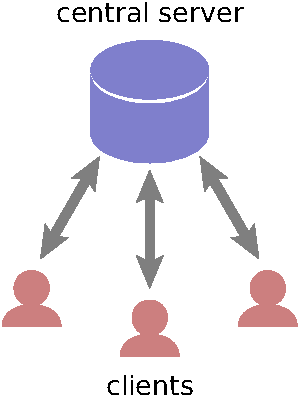
\includegraphics[width=\textwidth]{cvcs}
 \end{center}

 At any time, the central server contains well defined revisions
 of file sets which can be consecutively numbered.
\end{frame}

\begin{frame}{Distributed version control systems}
 \begin{center}
  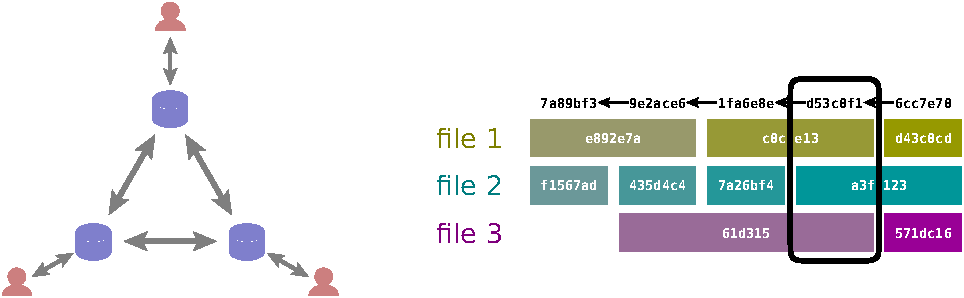
\includegraphics[width=\textwidth]{dvcs}
 \end{center}

 \begin{itemize}
  \item each individual repository has its own history
  \item each object is identified by a SHA1 hash consisting of
	40 hexadecimal values
  \item there are more than $10^{48}$ different SHA1 hashes
  \item often the first seven hex digits are sufficient for identification
 \end{itemize}
\end{frame}

\begin{frame}{Distributed VCS with Gitlab / Github}
 \begin{center}
  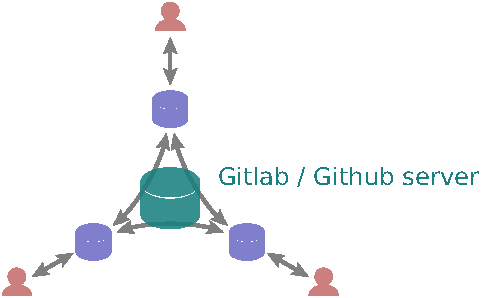
\includegraphics[height=0.6\textheight]{dvcs-github}
 \end{center}
\end{frame}

\begin{frame}{The prime time project}
 \textit{\structure{Question}}

 How many prime numbers can be interpreted as time in the format HH:MM?

 \vspace{1\baselineskip}
 \textit{\structure{Examples}}

 \textcolor{wrong}{2179 is a prime, but 21:79 is not a valid time}\\
 \textcolor{right}{2137 is a prime and 21:37 is a valid time}\\
 \textcolor{right}{953 is a prime and 9:53 is a valid time}\\
 \textcolor{wrong}{89 is a prime, but 0:89 is not a valid time}\\
 \textcolor{right}{41 is a prime and 0:41 is a valid time}\\
 \textcolor{right}{7 is a prime and 0:07 is a valid time}

 \vspace{1.5\baselineskip}
 \begin{center}
 \uncover<2>{\structure{\bfseries And, of course, we are going to use\\ a Git repository.}}
 \end{center}
\end{frame}

\begin{frame}[fragile]{Creating a respository}
 \structure{Initializing a new repository}

 \begin{lstlisting}
  ~/primetime$ git init
 \end{lstlisting}

 \vspace{\baselineskip}
 \structure{What has happened?}
 \begin{lstlisting}
  ~/primetime$ ls -a
  .  ..  .git
  ~/primetime$ ls .git
  branches  description  hooks  objects
  config    HEAD         info   refs
 \end{lstlisting}

 \begin{center}
  \uncover<2>{\alert{\raisebox{0.5em}{\dbend}\quad Keep your hands off the \texttt{.git} directory!!!}}
 \end{center}
\end{frame}

\begin{frame}[fragile]{Tell Git who you are}

 \structure{Specify your name and your email address}
 \begin{lstlisting}
  $ git config --global user.name <your name>
  $ git config --global user.email <your email>
 \end{lstlisting}

 \vspace{\baselineskip}
 \structure{\ldots and, if you want, your preferred editor}
 \begin{lstlisting}
  $ git config --global core.editor <editor>
 \end{lstlisting}

 \vspace{\baselineskip}
 \structure{example configuration}
 \begin{lstlisting}
  $ git config --list
  user.email=gert.ingold@physik.uni-augsburg.de
  user.name=Gert-Ludwig Ingold
  core.editor=vim
  ...
 \end{lstlisting}
\end{frame}

\begin{frame}[fragile]{It's prime time now}
 \texttt{primetime.py}
 \begin{lstlisting}
  def istime(n):
      hh, mm = divmod(n, 60)
      return 0 <= hh <= 23 and 0 <= mm <= 59

  print(sum(istime(n) for n in range(2360)))
 \end{lstlisting}

 \vspace{0.2truecm}
 \structure{What is the status?}
 \begin{lstlisting}[basicstyle={\ttfamily\tiny}, escapechar=\%]
  $ git status
  On branch master

  Initial commit

  Untracked files:
    (use "git add <file>..." to include in what will be committed)

	  %\textcolor{gitred}{primetime.py}%

  nothing added to commit but untracked files present (use "git add" to track)
 \end{lstlisting}
 \begin{itemize}
  \item Git has noticed our new file but ignores it
  \item Git tells us what to do in order to put the file under version control:
	\texttt{git add <file>}
 \end{itemize}
\end{frame}

\begin{frame}[fragile]{Adding a file}
 \begin{lstlisting}
  ~/primetime$ git add primetime.py
 \end{lstlisting}

 \vspace{0.2truecm}
 \structure{How did the status change?}
 \begin{lstlisting}[escapechar=\%]
  ~/primetime$ git status
 On branch master

 Initial commit

 Changes to be committed:
   (use "git rm --cached <file>..." to unstage)

         %\textcolor{gitgreen}{new file:}%   %\textcolor{gitgreen}{primetime.py}%
 \end{lstlisting}
 \begin{itemize}
  \item Our file is now in the staging area, \alert{it is not under version control yet!}
  \item Our file can now be committed, but we can add more files first
  \item Git tells us how we can remove the file from the staging area if we put
        it there by accident
 \end{itemize}
\end{frame}

\end{document}
